%!TEX root = ../main.tex
\vspace*{\fill}

{\large \bf Chapter~\ref{chp:angular} Authorship Statement}

\vspace{1em}


{\bf Citation:} Thomas Taimre, Patrick J.\ Laub (2018), \emph{Rare tail approximation using asymptotics and L1 polar coordinates}, Statistics and Computing (submitted)

\vspace{1em}

The authors of this paper equally contributed to the following tasks:
\begin{enumerate}
\item conception and design of the project;
\item mathematical arguments, and interpretation of the results;
\item writing the publication.
\end{enumerate}

In addition to this, I completed the majority of the computational work.

\vspace{3em}

\vspace*{\fill}

\chapter{Rare tail approximation using asymptotics and polar coordinates} \label{chp:angular}

\section{Introduction}

% A typical problem in the field of rare-event estimation is to find the probability
% \begin{equation} \label{ProbabilityOfInterest}
% \ell(\gamma) := \Prob(S > \gamma)
% \end{equation}
% where $S := X_1 + \dots + X_d$ for a fixed $d \in \NL$ and where the $\gamma \in \RL$ is large or increasing. In applications, we often wish to understand the behaviour of a combination of random factors, and hence the random variable (random variable) $S$ is ubiquitous in real-world modeling problems. It can model, for example: aggregate risk or portfolio value for holding $d$ risky assets \cite{mcneil2015quantitative,Rueschendorf2013}, the aggregate losses for $d$ insurance policy claims \cite{asmussen2010ruin,klugman2012loss}, the combined signal interference from $d$ wireless transmission sources \cite{fischione2007approximation}. Probabilities of the form \eqref{ProbabilityOfInterest} are used to understand how a system would behave under extreme scenarios such as a market crash, a power surge, or a natural disaster. One is typically interested not just in the quantity $\ell(\gamma)$ but in the behaviour of the summands when the extreme event $\{ S > \gamma \}$ occurs.

% This probability is available in closed-form for only a few basic cases, when the density of $S$ (which is an $d$-fold convolution) has a known closed-form solution, c.f. \cite{nadarajah2008review}. For example, when the summands are independent and identically distributed (iid) then it is sometimes simple to calculate (for exponential, gamma, normal, binomial, geometric, or negative binomial summands) and sometimes it is still intractable (for lognormal, Weibull, Cauchy, Laplace, Beta, or Chi-squared summands). However, requiring the assumption of independence (let alone iid-ness) of the summands is a stifling restriction when modeling real-world events; a notorious example would be the partial blame of the 2008--9 global financial crisis on mathematicians' inappropriate use of a simplistic dependence model (the Gaussian copula) \cite{salmon2009recipe}.

This chapter focuses on evaluating
\begin{equation} \label{ProbabilityOfInterest}
\ell(\gamma) := \Prob(S > \gamma)
\end{equation}
where $S := X_1 + \dots + X_d$ for a fixed $d \in \NL$ and where the $\gamma \in \RL$ is large or increasing. As detailed above, this is often a difficult problem which does not have a simple closed-form solution.

When analytical solutions are unavailable, the next best option is numerical integration, and after that Monte Carlo integration (or quasi-Monte Carlo).
Numerical integration algorithms applied to
\[ \ell(\gamma) = \int_{\RL^d} \ind{ x_1 + \dots + x_d > \gamma} f_{\bfX}(\bfx) \dd \bfx \]
are typically slow, inaccurate, and misleading. This is because the indicator is rarely 1, floating-point errors accumulate, and the curse of dimensionality applies for $d$ larger than about 2 or 3. Some of these algorithms attempt to estimate the error in their result, but there are few (if any) theoretical guarantees that these estimates are reliable.

Rare-event problems also cause difficulties for the crude Monte Carlo (CMC) estimator. This is obvious as the CMC estimator's relative error explodes for large $\gamma$ --- that is, the CMC estimator $\hat{\ell}_{\text{CMC}}(\gamma) := \ind{S > \gamma}$ has
\[ \lim_{\gamma \to \infty} \text{RelativeError}\{ \hat{\ell}_{\text{CMC}}(\gamma) \} = \lim_{\gamma \to \infty} \frac{ \Var[ \hat{\ell}_{\text{CMC}}(\gamma) ] }{ \ell(\gamma)^2 } = \lim_{\gamma \to \infty} \frac{  \ell(\gamma)[1-\ell(\gamma)] }{  \ell(\gamma)^2 } = \infty \,. \]
Intuitively, the problem is because the indicator $\ind{S > \gamma}$ is eventually always 0 when $\gamma$ gets very large. In response, various variance reduction techniques have been applied so that there are now a large collection of estimators with better performance in this setting, c.f. `rare-event estimation' in \cite{kroese2013handbook,asmussen2007stochastic,glasserman2003monte}.

There is, of course, no silver bullet for the problem. Some estimators only apply to specific distributions (e.g. \cite{botev2017fast} for sums of lognormals, \cite{yao2016estimating} for sums of phase-type mixtures) or to certain classes of distributions (exponential tilting for light-tailed summands \cite{kroese2013handbook,asmussen2007stochastic}, hazard-rate twisting or the Asmussen--Kroese method \cite{asmussen2006improved} for heavy-tailed summands). Other estimators are general but require specifying either some extra information (e.g. some conditional distributions for conditional Monte Carlo \cite{asmussen2017conditional}, or a sampling distribution for importance sampling). The most general estimators --- such as the generalised splitting method, cross-entropy method, or Markov Chain Monte Carlo (MCMC) methods like \cite{chan2012improved} --- are usually computationally demanding, they often depend upon an intelligent selection of input parameters to perform efficiently, and are somewhat complicated.

While we almost never have an analytic solution for $\ell(\gamma)$, it is somewhat common to know the \emph{asymptotic approximation} to it, and this forms the basis for our proposed estimator. For example, if $\bfX \sim \mathsf{Lognormal}(\bfmu, \bfSigma)$ where $\bfmu \in \RL^d$ and $\bfSigma \in \RL^{d \times d}$ is positive definite, then it has been shown that \cite{asmussen2008asymptotics}
\begin{equation} \label{SLNasymptotic}
\ell(\gamma) = \Prob(S > \gamma) \sim \sum_{i=1}^d \Prob(X_i > \gamma) \qquad \text{ as } \gamma \to \infty
\end{equation}
where $f(x) \sim g(x)$ denotes $\lim_{x \to \infty} f(x)/g(x) = 1$. Thus, one is tempted to label the RHS of \eqref{SLNasymptotic} as $\hat{\ell}_{\mathrm{Asym}}(\gamma)$ and use it as an approximation for $\ell(\gamma)$. For certain values of $(\bfmu,\bfSigma)$ this asymptotic approximation can be accurate, in others it can be wildly inaccurate, depending on how fast the asymptotic approximation converges to the true value; see Figure~\ref{fig:slow_convergence} for an illustration where it is only when $\ell(\gamma) \lesssim 10^{-10}$ that the asymptotic form begins to give accurate estimates (i.e., $\hat{\ell}_{\mathrm{Asym}}(\gamma) / \ell(\gamma) > 0.99$). A discussion of this phenomenon is in \cite{botev2017fast}.

\begin{figure}
\centering
\includegraphics[width=.95\textwidth]{"Lognormal Asymptotic Comparison"}
\caption{A comparison of $\ell(\gamma)$ and $\hat{\ell}_{\text{Asym}}(\gamma)$ for $X_1+X_2$ where $X_1 \sim \LNDist(0, 1)$ is independent to $X_2\sim\LNDist(0,\frac{3}{4})$. The $y$ axis plots $\hat{\ell}_{\text{Asym}}(\gamma) / \ell(\gamma)$, and the $x$ axis shows ${-}\log_{10} \ell(\gamma)$. The two lines describe two possible asymptotics, the yellow ``Two terms'' describes $\hat{\ell}_{\text{Asym}}(\gamma)$ as given in \eqref{SLNasymptotic} whereas the blue ``One Term'' uses just the first term of this sum.}
\label{fig:slow_convergence}
\end{figure}

We propose an \emph{importance sampling} estimator which incorporates the asymptotic approximation and uses Monte Carlo sampling to estimate the difference between $\ell(\gamma)$ and $\hat{\ell}_{\mathrm{Asym}}(\gamma)$. In the estimator, the asymptotic approximation acts like a prior belief (though it is just a point-estimate) of the value of $\ell(\gamma)$, which gets corrected/updated with more samples.

The main drawback to importance sampling is \emph{likelihood degeneration}, where one can face numerical errors if $\gamma$ or $d$ is extremely large.
The degeneration caused by a large $d$ is only partially compensated by our method, so we take $d \le 100$.
To mitigate degeneration for large $\gamma$, we focus our attention of values of $\gamma$ which are moderately large but not unrealistically so.
Our goal is to provide an estimator which is practically useful when $\ell(\gamma)$ is between roughly $10^{-3}$ and $10^{-7}$.%; one motivation comes from the US Nuclear Regulatory Commission uses a ``95/95'' rule, where decisions are made based on the upper 95\% confidence interval for a 95\% quantile of a random quantity \cite{lurie2011applying}.

The range of probabilities that we consider are unusual as they are less rare than much of the standard rare-event literature. The orthodox approach is to construct an estimator $\hat{\ell}(\gamma)$ and analyse the limit $\lim_{\gamma\to\infty} \Var(\hat{\ell}(\gamma))/\ell(\gamma)^2$; if the limit is small (i.e., zero, bounded, or at least grows only at a polynomial rate) then the estimator is branded as a success (it has `vanishing relative error', `bounded relative error', or is `logarithmically efficient' respectively) regardless of its behaviour in the finite $\gamma$ situation. It can happen that these desirable limiting properties are only discernible in cases when the probabilities are truly minuscule (e.g. of order $10^{-10}$ or smaller); in a situation like this, the model error would surely dominate any estimation error.

The estimator is introduced in Section~\ref{scn:Estimator}, the results from numerical comparisons are in Section~\ref{Sec:Results}, and Section~\ref{Sec:Conclusion} concludes the discussion.

\section{The polar estimator} \label{scn:Estimator}

\subsection{The general form}

We construct an estimator of the quantity $\ell(\gamma) := \Prob(S > \gamma)$, where $S = X_1 + \dots + X_d$ for large $\gamma$ by applying IS.
Standard IS theory says to construct an estimator which samples from a distribution close to $f_{\bfX \,|\, S>\gamma}$ (that is, the distribution of $\bfX$ conditioned on $\{ S>\gamma \}$), rather than the original $f_{\bfX}$. To do this, perform a change of variables so
\[ \bfX \longrightarrow (S,\bfTheta) := \left(X_1+\dots+X_d, \bfX / [X_1+\dots+X_d] \right) \,. \]
The new density $f_{(S,\bfTheta)}$ is available (if $f_{\bfX}$ is known), and is
\[
f_{(S,\bfTheta)}(s,\bftheta) = f_{\bfX}(s\bftheta) \times |s|^{d-1}\,.
\]

Consider IS in this new form. Imagine that we have a density $g_{(S,\bfTheta)}$ which is in some way similar to $f_{(S,\bfTheta)}$, and we also know the marginal density $g_S(s) := \int g_{(S,\bfTheta)}(s,\bftheta) \dd \bftheta$ and the conditional density $g_{\bfTheta \mid S}:=g_{(S,\bfTheta)}/g_S$. If we truncate $g_{(S,\bfTheta)}$ so that $S>\gamma$ a.s., and use this as the IS measure, we get
\begin{equation} \label{eq:general_form_estimator}
\hat{l}_{\mathrm{IS}}(\gamma) := \frac{\overline{G}_S(\gamma)}{R} \sum_{r=1}^R \frac{ f_{(S,\bfTheta)}(S^{[r]}, \bfTheta^{[r]}) }{ g_S( S^{[r]} ) g_{\bfTheta \mid S}(\bfTheta^{[r]}\,|\, S^{[r]})}
\quad \text{for} \quad
\genfrac{}{}{0pt}{}{ S^{[r]} \iidDist g_{S \mid S>\gamma}, }{ \bfTheta^{[r]} \indDist g_{\bfTheta \mid S}( \,\cdot\, | S^{[r]}), }
\end{equation}
where $\overline{G}_S(\gamma) :=  \int_{\gamma}^\infty g_S(s) \dd s$, and $g_{S \mid S>\gamma}:=g_S \ind{ S>\gamma } / \overline{G}_S(\gamma)$.

We investigate estimators of the general form of \eqref{eq:general_form_estimator} which we call \emph{polar estimators}.
These are accurate when $g_{(S,\bfTheta)}= g_S \times g_{\bfTheta \mid S}$ closely resembles $f_{(S,\bfTheta)}=f_S \times f_{\bfTheta \mid S}$.
This is done in two steps, by finding a \emph{radial approximation} $g_S$ which approximates $f_S$, and an \emph{angular approximation} $g_{\bfTheta \mid S}$ similar to $f_{\bfTheta \mid S}$, problems we discuss in the following sections.


\subsection{The radial approximation}

As mentioned in the introduction, we consider utilising the asymptotic form of the sum in our estimator --- they form our radial approximation. To clarify the notation, we again define the relevant asymptotic forms:

\begin{definition}[Asymptotic form]
If for some function $\Asymf \in \Lp^1(\RL)$, with tail $\AsymFTail(s) = \int_s^\infty \Asymf(x) \dd x$, and constant $c_S \in \RL_+$, we have that
\begin{equation} \label{asymptotic_sum}
  f_S(s)\ \sim\ c_S \Asymf(s) \for{s \to \infty}
\end{equation}
then we say $\Asymf$ is an \emph{asymptotic form} of $f_S$. \remQED
\end{definition}

Thus, in the general form \eqref{eq:general_form_estimator} we will use $g_S = \Asymf$ when it is available and is a proper pdf. There are some technicalities for the cases when $\Asymf$ does not form a proper pdf which we defer for now.
The estimator resulting from this radial approximation is
\begin{equation} \label{eq:asymptotic_estimator}
\hat{l}_{\mathrm{IS2}}(\gamma) := \frac{c_S \AsymFTail(\gamma)}{R} \sum_{r=1}^R \frac{ f_{(S,\bfTheta)}(S^{[r]}, \bfTheta^{[r]}) }{ c_S \Asymf( S^{[r]} )g_{\bfTheta \mid S}(\bfTheta^{[r]}\,|\, S^{[r]})}
\quad \text{for} \quad
\genfrac{}{}{0pt}{}{S^{[r]} \iidDist \AsymfTrun, }{ \bfTheta^{[r]} \indDist g_{\bfTheta \mid S}( \,\cdot\, | S^{[r]}). }
\end{equation}

\begin{remark}
Define $\mathcal{R}(\gamma)$ by
$ \ell(\gamma)~=~\hat{\ell}_{\mathrm{Asym}}(\gamma) \mathcal{R}(\gamma) $; n.b.\ $\hat{\ell}_{\mathrm{Asym}}(\gamma) := c_S \AsymF(\gamma)$.
We can see that $\hat{\ell}_{\mathrm{IS2}}(\gamma)$ has a nice interpretation, because
\[ \hat{\ell}_{\mathrm{IS2}}(\gamma) = \hat{\ell}_{\mathrm{Asym}}(\gamma) \times \hat{\mathcal{R}}(\gamma) \,, \]
where $\hat{\mathcal{R}}(\gamma)$ is a Monte Carlo estimate of $\mathcal{R}(\gamma)$. \remQED
\end{remark}

The recent applied probability literature has found the $\Asymf$ for a staggering array of distributions of $\bfX$. Perhaps the simplest case is when the $X_i$ are iid subexponential random variables. By definition (cf. \cite{foss2011introduction}), they satisfy
\begin{equation} \label{Subexponential_Asymptotics_IID}
f_S(s)\ \sim\ d \, f_1(s) \for{s \to \infty}\,.
\end{equation}
For sums of independent non-identically distributed subexponential variables (or for sums containing some subexponential and some lighter-tailed variables) we have
\begin{equation} \label{Subexponential_Asymptotics_Non_IID}
f_S(s)\ \sim\ \sum_{i=1}^d f_i(s)\ \sim\ \sum_{i\in I} f_i(s) \for{s \to \infty}
\end{equation}
where $I$ is the set of indices of slowest tail decay. The asymptotics in \eqref{Subexponential_Asymptotics_Non_IID} also hold in many regimes where dependence has been introduced, cf. \cite{foss2010sums,wuthrich2003asymptotic,alink2004diversification,alink2007diversification}.

A distribution can satisfy a stronger property called \emph{regular variation} which implies subexponentiality and hence the asymptotics above. Examples of regularly varying distributions are Cauchy, Fr\'{e}chet, and Pareto distributions \cite{bingham1989regular}. The lognormal and heavy-tailed Weibull distributions are subexponential but not regularly varying.

The Weibull distribution is interesting as it is a family which can be heavy-tailed, light-tailed (the Raleigh distribution is a special case), or on the boundary between these (i.e. the exponential distribution). The asymptotic form for the heavy-tailed Weibull sum is covered by \eqref{Subexponential_Asymptotics_IID} and \eqref{Subexponential_Asymptotics_Non_IID} as the summands are subexponential. The difficulty in finding the asymptotics for the light-tailed case led the authors to investigate it in detail, leading to the paper \cite{asmussen2017tail} which uses results originally from \cite{balkema1993densities}.

\begin{proposition} \label{prop:light_weibull} Assume that $X_1, \dots, X_d$ are iid light-tailed $\mathsf{Weibull}(\beta, \lambda)$ where $\beta>1$, $\lambda \in \RL_+$, $d \ge 2$. Then
\begin{equation*}
F_S(s)\ \sim\ \Bigl[ \frac{2\beta\pi}{\beta-1}\Bigr]^{(d-1)/2} d^{-1/2} \Big( \frac{s}{\lambda d} \Big)^{\beta(d-1)/2} \Ftail \Big( \frac{s}{d} \Big)^d \for{s \to \infty}\,.
\end{equation*}
\end{proposition}

The exposition in \cite{asmussen2017tail} details this and more general asymptotics (i.e.\ the independent but non-identically distributed case, and when the variables are not exactly Weibull but are `Weibull-like').

\subsection{The angular approximation}

The choice of angular approximation is not as obvious as was the choice of radial approximation.
Finding a conditional density $g_{\bfTheta \mid S}$ which is similar to $f_{\bfTheta \mid S}$ has little to no precedent in the literature.

We can make a simplification by looking at a different conditional distribution. Instead of taking an $S$ which is larger than $\gamma$ and asking `what is the distribution of $\bfTheta$ given this $S$?', we can instead ask `what is the distribution of $\bfTheta$ given $S > \gamma$?'. This second conditional will resemble the first when $\gamma$ becomes large, since it is typically the case that $\Exp[ S-\gamma \mid S > \gamma]$ converges quickly to zero.
Also we have a computation benefit to finding a $g_{\bfTheta \mid S > \gamma}$ which is similar to $f_{\bfTheta \mid S > \gamma}$ as this distribution will be constant across all Monte Carlo iterates, in contrast to $g_{\bfTheta \mid S^{[r]}}$ and $f_{\bfTheta \mid S^{[r]}}$.

When it is possible, we follow the same approach as the radial approximation and utilise some asymptotic information. However, if one re-uses the previous asymptotic form, that is
\[ f_{\bfTheta \mid S}(\bftheta | s) = \frac{f_{S,\bfTheta}(s, \bftheta)}{f_S(s)} \sim \frac{f_{\bfX}(s \bftheta) |s|^{d-1}}{\Asymf(s)} =: g_{\bfTheta \mid S}(\bftheta | s) \,, \]
which is natural, then the estimator \eqref{eq:asymptotic_estimator} degenerates to the deterministic
\begin{equation*} \label{eq:double_asymptotic_estimator}
\hat{l}_{\mathrm{IS2}}(\gamma) := \frac{\AsymFTail(\gamma)}{R} \sum_{r=1}^R 1 = \AsymFTail(\gamma) \,.
\end{equation*}

Unfortunately, the conditional $f_{\bfTheta \mid S}$ and $f_{\bfTheta \mid S}$ distributions are rarely examined in the literature, so we do not have a ready supply of their asymptotics.

When the summands are subexponential, then the distribution of $(\bfTheta \mid S = s)$ as $s\to\infty$ degenerates to a discrete distribution over the unit vectors $\bfe_1$, \dots, $\bfe_d$. This is just a re-casting of the principle of the single big jump (cf.\ Section~\ref{sec:asymptotics} or \cite{foss2011introduction}). One density, which we call the \emph{optimistic density} (see the algorithm below), that is asymptotically equivalent to $(\bfTheta \mid S = s)$ is
\begin{align} \label{OptimisticPDF}
g_{\bfTheta \mid S}(\bftheta \mid s)
&= |s|^{d-1} \sum_{i=1}^d p_i(s) f_{\bfX_{-i}}(s \bftheta_{-i}) \ind{ \theta_i = 1-\bfone \cdot \bftheta_{-i} }
\end{align}
where the $p_i$ functions are defined by
\begin{equation} \label{optim_pi}
p_i(s) = \frac{\Ftail _i(s)}{\sum_{j=1}^d \Ftail _j(s)} \,.
\end{equation}
Algorithm~\ref{Alg:Optimism} shows a method for sampling from this $g_{\bfTheta \mid S}(\bftheta \mid s)$, and Proposition~\ref{prop:optimistic_asymptotic} shows has the expected limiting distribution as $s \to \infty$.

\begin{algorithm}[H]
\caption{Sampling from the optimistic angular density}\label{Alg:Optimism}
\begin{algorithmic}[1]
\Procedure{Optimistic}{$s$, $F_1$, \dots, $F_d$}
\State Simulate index $I$ in $\{1, \dots, d\}$ by $\Prob(I=i) = p_i(s)$ from \eqref{optim_pi}.
\For{$i = 1$ \textbf{to} $d$ \textbf{except} $I$}
\State $X_i^* \gets$ Random sample from $F_i$
\EndFor
\State $X_I^* \gets s - \sum_{i \not= I} X_i$ \Comment{This can be negative, but we are optimistic}
\State \textbf{return} $\bfTheta \gets \bfX^* / s$
\EndProcedure
\end{algorithmic}
\end{algorithm}

\begin{proposition} \label{prop:optimistic_asymptotic}

The optimistic density \eqref{OptimisticPDF} converges as $s \to \infty$ to the singular density
\begin{equation} \label{OptimisticLimitingDensity}
g_\infty(\bftheta) := \sum_{i=1}^{d} p_i \, \ind { \bftheta = \bfe_i } \,,
\end{equation}
where $p_i = \lim_{s\to\infty} p_i(s)$ for $i=1,\dots,d$.
\end{proposition}

\begin{proof}
For some $\bft=(t_1,\dots,t_d)' \in \mathbb{R}^d$, the characteristic function of $g_{\bfTheta \mid  S}$ is
\[
\phi_{g_{\bfTheta \mid  S}}(\bft \mid s)
= \Exp \exp\left(\ih\,\bft^\top \bfTheta \right)
= \Exp \left[ \exp\left(\ih\,\frac{\bft}{s}^\top \bfX^* \right) \right]
\]
where $\bfX^* = s \bfTheta$ as in Algorithm~\ref{Alg:Optimism}.

So, with $I$ as the discrete variable defined in Algorithm~\ref{Alg:Optimism}, we have
\begin{align*}
\phi_{g_{\bfTheta \mid  S}}(\bft \mid s)
&= \sum_{j=1}^d p_j(s) \Exp \left[ \exp\left(\ih\,\frac{\bft}{s}^\top \bfX^* \right) \,\Big|\, I = j \right] \\
&= \sum_{j=1}^d p_j(s) \Exp \left[ \exp \left\{ \ih \left[ \frac{\bft_{-j}}{s}^\top \bfX^*_{-j} + \frac{t_j}{s} (s - \bfone^\top \bfX^*_{-j}) \right] \right\}  \,\Big|\, I = j \right] \\
&= \sum_{j=1}^d p_j(s) \e^{\ih t_j} \Exp \left[ \exp\left(\ih\,\frac{(\bft_{-j} - t_j \bfone)}{s}^\top \bfX_{-j} \right)  \right] \\
&= \sum_{j=1}^d p_j(s) \e^{\ih t_j} \phi_{\bfX_{-j}} \left(  \frac{(\bft_{-j} - t_j \bfone)}{s} \right) \,.
\end{align*}
Therefore,
\[
\lim_{s \to \infty} \phi_{g_{\bfTheta | S}}(\bft ; s)
= \sum_{j=1}^d p_j \e^{\ih t_j}
= \sum_{j=1}^d p_j \e^{\ih \bft^\top \bfe_j}
\]
which has the singular density as in \eqref{OptimisticLimitingDensity}.
\end{proof}

\begin{remark}
The polar estimator with the optimistic angular approximation \eqref{OptimisticPDF} simplifies to
\[
\hat{l}_{\mathrm{IS2}}(\gamma)
= \frac{c_S \AsymFTail(\gamma)}{R} \sum_{r=1}^R \frac{\mathrm{HarmonicMean}( f_{X_1}( S^{[r]} \Theta^{[r]}_1), \dots, f_{X_d}( S^{[r]} \Theta^{[r]}_d) )}{c_S \Asymf( S^{[r]} )}
\]
where $S^{[r]} \iidDist \AsymfTrun$, $\bfTheta^{[r]} \indDist g_{\bfTheta \mid S}( \,\cdot\, | S^{[r]})$. \remQED
\end{remark}

The conditional angular asymptotic distribution is harder to obtain in the case of light-tailed summands. The following example shows these distributions differ qualitatively when different copulas are considered.

\begin{example}
Consider $X_1$ and $X_2$ are \textsf{Exp}(1) variables which are: i) independent, ii) \textsf{Clayton}(1) dependent, or iii) \textsf{Ali-Mikhail-Haq}(-1) dependent. The sum densities are
\[ f_S^{\mathrm{Ind}}(s) = s \e^{-s} \quad \text{for } s > 0 \,, \]
\[ f_S^{\mathrm{Cla}}(s) = \frac{2 - 2 \cosh(s) + s \sinh(s)}{(\cosh(s)-1)^2} \quad \text{for } s > 0 \]
\[ f_S^{\mathrm{AMH}}(s) = 8 \csch(s)^3 \sinh(s/2)^4 \quad \text{for } s > 0 \]
respectively, and hence for $s>0$ and $\theta \in (0,1)$
\[ f^{\mathrm{Ind}}_{\Theta_1 | S}(\theta | s) = 1 \,, \]
\[ f^{\mathrm{Cla}}_{\Theta_1 | S}(\theta | s) = \frac{ s \e^{-s \theta}(\e^s - \e^{s \theta})(\e^{s \theta}-1)}{2 + s - 2\e^s + s \e^s} \,, \]
\[ f^{\mathrm{AMH}}_{\Theta_1 | S}(\theta | s) = \frac{ s \e^{-s \theta}(\e^s + \e^{2 s \theta})}{2(\e^s - 1)}  \]
respectively. It is interesting to note that the asymptotic independence of the Clayton copula would indicate that $f^{\mathrm{Cla}}_{\Theta_1 | S}(\theta | s) / f^{\mathrm{Ind}}_{\Theta_1 | S}(\theta | s) \to 1$ as $s\to\infty$ which is almost the case ($f^{\mathrm{Cla}} /  f^{\mathrm{Ind}} \to 2$). In contrast, $f^{\mathrm{AMH}}_{\Theta_1 | S}(\theta | s)$ degenerates to a pair of atoms at 0 and 1 as $s \to \infty$. %, see:
% \begin{figure}[H]
% \centering
% 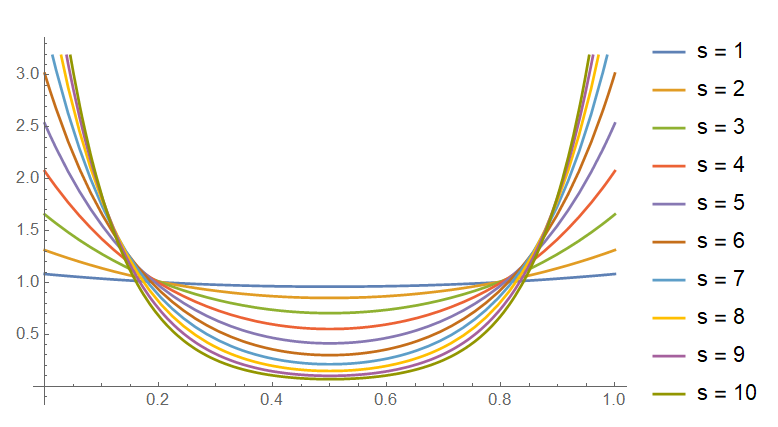
\includegraphics[width=0.7\textwidth]{amh.png}
% \end{figure}
\end{example}

% \begin{example}

% % \begin{align*}
% %     f(\bftheta | s) &= \frac{f_{\bfX}(s \bftheta) s^{d-1}}{ f_S(s) } \\
% %     &= \frac{ c( F_1(s \theta_1), \dots, F_d(s \theta_d)) \prod_{i=1}^d f_{X_i}(s \theta_i) s^{d-1}}{ f_S(s) } \times \frac{ f_{S_{Ind}}(s) }{ f_{S_{Ind}}(s) } \\
% %     &= c( F_1(s \theta_1), \dots, F_d(s \theta_d)) \times \frac{  \prod_{i=1}^d f_{X_i}(s \theta_i) s^{d-1} }{ f_{S_{Ind}}(s)} \times \frac{ f_{S_{Ind}}(s) } { f_S(s) } \\
% % \end{align*}

% For the $\mathsf{Exp}(1)$ case, we have%\footnote{Note sure if this is true for all copulas, or just for all copulas with these marginals, or just for all copulas with the same marginals, or\dots}
% \[ \frac{  \prod_{i=1}^d f_{X_i}(s \theta_i) s^{d-1} }{ f_{S_{Ind}}(s)} = 1 \qquad \text{for all valid } \bftheta \]
% For the $\mathsf{Clayton}(1)$ copula, we have
% \[ \frac{ f_{S_{\mathrm{Ind}}}(s) } { f_S(s) } = \frac{s e^{-s} (\cosh (s)-1)^2}{s \sinh (s)-2 \cosh (s)+2}  \]
% which goes to $1/2$ as $s \to \infty$. \\
% For the $\mathsf{AMH}(-1)$ copula, we have
% \[ \frac{ f_{S_{\mathrm{Ind}}}(s) } { f_S(s) } = \frac{1}{8} s e^{-s} \sinh ^3(s) \text{csch}^4\left(\frac{s}{2}\right)
%   \]
% which goes to $\infty$ as $s \to \infty$.
% \hfill $\Diamond$
% \end{example}

One (light-tailed) case where we can find an asymptotic angular distribution is for light-tailed Weibull sums. The angular asymptotic can be extracted from the following result in \cite{asmussen2017tail}.

\begin{proposition} \label{prop:light_weibull_angles}
Say $X_1, \dots, X_d$ are iid light-tailed $\mathsf{Weibull}(\beta, 1)$ with survival function $\Ftail(x)=\e^{-x^\beta}$ where $\beta>1$, $d \ge 2$.
Define the vector function $\bfW(x)$ component-wise by
\[ W_i(x) = \omega(x) ( X_i - x/d) \,, \quad \text{ for } i=1,\dots,d\,, \]
where $\omega(x) := \sqrt{2  \beta (\beta-1) (x/d)^{\beta-2}}$.
Then as $\gamma \to \infty$ we have
\[ (\bfW(\gamma) \mid S > \gamma) \convdistr \NormDist\left(\bfzero, (1 - \rho) \bfI + \rho \right) \,,\]
where $\rho = -1/(d-1)$.
\end{proposition}

% In the subexponential case, we conjecture that the following simulates from the asymptotic angular distribution:

%\begin{Conjecture}
%Assume that $X_1, \dots, X_d$ are independent non-identically distributed positive subexponential r.v.'s with cdfs $F_1$, \dots, $F_d$.
%Given $S = s$, define $I$ as a random variable in $\{1, \dots, d\}$ with $\Prob(I=i) \propto \Ftail _i(s)$. An asymptotic form of $\bfTheta \mid S=s$ is
%\begin{equation} \label{OptimisticPDF}
%g_{\bfTheta \mid S}(\bftheta \mid s) = \sum_{i=1}^d  \Prob(I = i) \prod_{j\not=i} f_{X_j}(s \, \theta_j) \,.
%\end{equation}
%\end{Conjecture}
%\begin{proof}
%TODO: Prove this bad boy then rename from conjecture to theorem.
%\end{proof}







% Notation.  Write $\bftheta=(\theta_1,\dots,\theta_d)$ with $\theta_d := 1-\sum_{j=1}^{d-1}\theta_j$.

% Write $\bfone_k$ for a $k\times 1$ vector of all ones.
% Write $\bfzero_k$ for a $k\times 1$ vector of all zeros.
% Write $\bfe^{(k)}_i$ for a $k\times 1$ vector of zeros with a single one in the $i$-th position.
% Write $I_k$ for the $k\times k$ identity matrix.
% Write $Z_{m,n}$ for the $m\times n$ matrix of zeros.  In the case of a square matrix, write simply $Z_k := Z_{k,k}$.

% For a $k\times 1$ vector $\bfv$, $v^{(-i)}$ is the $(k-1)\times 1$ vector with $i$-th element removed.
% For an $m\times n$ matrix $A$, $A^{(-i)}$ is the $(m-1)\times n$ matrix with $i$-th row removed.




% Write $\bftheta^{(-i)}$ for $\bftheta$ with $i$-th element removed.


% \begin{proof}
% Fix the $(d-1)$ independent variables as $\bftheta^{(-d)}$.
% For some $\mathbf{t}=(t_1,\dots,t_{d-1})' \in \mathbb{R}^{d-1}$, the characteristic function of
% the limiting random variable is
% \[
% \phi_\infty(\mathbf{t}) := \Exp_{g_\infty} \exp\left(\ih\,\mathbf{t}' \bfTheta^{(-d)} \right) = p_d(s) + \sum_{i=1}^{d-1} p_i(s) \e^{\ih\,t_i}\,.
% \]
% For the characteristic function corresponding to \eqref{OptimisticPDF}, we have
% \[
% \phi_s(\mathbf{t}) := \Exp_{g_{\bfTheta \mid S}} \exp\left(\ih\,\mathbf{t}' \bfTheta^{(-d)} \right) =\sum_{i=1}^d p_i(s) \frac{\int_{\mathbb{S}^{d-1}} \e^{\ih\,\mathbf{t}' \bftheta^{(-d)}}\,\prod_{j\not=i} f_{j}(s \, \theta_j) \dd \bftheta }{\int_{\mathbb{S}^{d-1}} \prod_{j\not=i} f_{j}(s \, \theta_j) \dd \bftheta}\,.
% \]
% For each $i=1,\dots,d$, consider a single term in the sum.
% Apply the following transformation of variables to both integrals in the numerator and denominator.

% Let $\mathbf{a} := \bfe_d^{(d)}$ and
% \[
% B = \begin{pmatrix}
% I_{d-1}\\
% -\bfone_{d-1}'
% \end{pmatrix}\,.
% \]
% Change variables as
% \[
% \bfv^{(i)} = s \bftheta^{(-i)} = s\left( \mathbf{a}^{(-i)} + B^{(-i)} \bftheta^{(-d)} \right)\,,
% \]
% so that
% \[
% \bftheta^{(-d)} = \left(B^{(-i)}\right)^{-1} \left( s^{-1} \, \bfv^{(i)} - \mathbf{a}^{(-i)} \right)\,.
% \]
% Note that, if $i=d$ then $\left(B^{(-i)}\right)^{-1} = I_{d-1}$, otherwise for $i=1,\dots,d-1$ we have
% \[
% \left(B^{(-i)}\right)^{-1} =
% \begin{pmatrix}
% I_{i-1} & Z_{i-1,d-i-1} & \bfzero_{i-1}\\
% & - \bfone_{d-1}' & \\
% Z_{d-i-1,i-1} & I_{d-i-1} & \bfzero_{d-i-1}\\
% \end{pmatrix}\,,
% \]
% so that in particular we have $ - \left(B^{(-i)}\right)^{-1} \mathbf{a}^{(-i)} = \bfe_i^{(d-1)}$ for $i=1,\dots,d-1$
% and $- \left(B^{(-d)}\right)^{-1} \mathbf{a}^{(-d)} = \bfzero_{d-1}$.
% For fixed $s$, under these changes of variables, we have
% \[
% \phi_s(\mathbf{t}) %= \sum_{i=1}^d p_i(s) \frac{\int_{s\,\mathbb{S}^{d-1}} s^{-1} \, \e^{\ih\,\mathbf{t}' \left(B^{(-i)}\right)^{-1} \left( s^{-1} \, \bfv^{(i)} - \mathbf{a}^{(-i)} \right)}\,\prod_{j\not=i} f_{j}(v^{(i)}_{j-\ind(j>i)}) \dd \bfv^{(i)}}{\int_{s\,\mathbb{S}^{d-1}} s^{-1} \, \prod_{j\not=i} f_{j}(v^{(i)}_{j-\ind(j>i)}) \dd \bfv^{(i)}}
% = \sum_{i=1}^d p_i(s) \frac{\e^{\ih\,\mathbf{t}'  \left( \ind(i\not=d)\bfe_i^{(d-1)} + \ind(i=d) \bfzero_{d-1}\right)}\,\int_{s\,\mathbb{S}^{d-1}} \e^{\ih\,\mathbf{t}'  \left( s^{-1} \, \left(B^{(-i)}\right)^{-1} \bfv^{(i)}\right)}\,\prod_{j\not=i} f_{j}(v^{(i)}_{j-\ind(j>i)}) \dd \bfv^{(i)}}{\int_{s\,\mathbb{S}^{d-1}} \prod_{j\not=i} f_{j}(v^{(i)}_{j-\ind(j>i)}) \dd \bfv^{(i)}}\,.
% \]
% Notice that, as $s\to\infty$, $s\,\mathbb{S}^{d-1} \to \mathbb{R}^{d-1}$.
% Moreover, for fixed $\mathbf{t}$, as all terms remain bounded for any $s>0$, we may freely exchange a limits and integrals as $s\to\infty$.
% Thus, we have
% \[
% \lim_{s\to\infty} \phi_s(\mathbf{t}) =
% \sum_{i=1}^d p_i \frac{\e^{\ih\,\mathbf{t}'  \left( \ind(i\not=d)\bfe_i^{(d-1)} + \ind(i=d) \bfzero_{d-1}\right)}\,\int_{\mathbb{R}^{d-1}} \lim_{s\to\infty} \e^{\ih\,\mathbf{t}'  \left( s^{-1} \, \left(B^{(-i)}\right)^{-1} \bfv^{(i)} \right)}\,\prod_{j\not=i} f_{j}(v^{(i)}_{j-\ind(j>i)}) \dd \bfv^{(i)}}{\int_{\mathbb{R}^{d-1}} \prod_{j\not=i} f_{j}(v^{(i)}_{j-\ind(j>i)}) \dd \bfv^{(i)}}\,,
% \]
% which is
% \[
% \lim_{s\to\infty} \phi_s(\mathbf{t}) =
% \sum_{i=1}^d p_i \frac{\e^{\ih\,\mathbf{t}'  \left( \ind(i\not=d)\bfe_i^{(d-1)} + \ind(i=d) \bfzero_{d-1}\right)}\,\int_{\mathbb{R}^{d-1}} \prod_{j\not=i} f_{j}(v^{(i)}_{j-\ind(j>i)}) \dd \bfv^{(i)}}{\int_{\mathbb{R}^{d-1}} \prod_{j\not=i} f_{j}(v^{(i)}_{j-\ind(j>i)}) \dd \bfv^{(i)}}\,,
% \]
% which further reduces to
% \[
% \lim_{s\to\infty} \phi_s(\mathbf{t}) =
% \sum_{i=1}^d p_i \e^{\ih\,\ind(i\not=d)t_i}\,,
% \]
% or in other words $\lim_{s\to\infty} \phi_s(\mathbf{t}) = \phi_\infty(\mathbf{t})$ pointwise, and as $\phi_\infty$ is continuous at the origin,
% we have the required convergence in distribution.
% \end{proof}

% Let's check if the density of $\bfX^*$ is correct. First split up
% \[ \mathcal{S}_+(s) = \{ \RL_+^d : \bfone \cdot \bfx = s \} , \quad
%    \mathcal{S}_-(s) = \{ \RL^d : \bfone \cdot \bfx = s, \bfx_{[1]}<0 \} \]
% so $\mathcal{S}(s)$ is partitioned by $\mathcal{S}_+(s)$ and $\mathcal{S}_-(s)$.

% \begin{align*}
% &~\int_{\bfx \in \mathcal{S}(s)}
% \sum_{i=1}^d p_i(s) f_{\bfX_{-i}}(\bfx_{-i}) \delta_{\{x_i = s - \bfone \cdot \bfx_{-i} \}} \dd \bfx \\
% &= \sum_{i=1}^d p_i(s)  \int_{\bfx \in \RL^d}
% f_{\bfX_{-i}}(\bfx_{-i}) \delta_{\{x_i = s - \bfone \cdot \bfx_{-i} \}} \dd \bfx \\
% &= \sum_{i=1}^d p_i(s)  \int_{\bfx_{-i} \in \RL_+^{d-1}}
% f_{\bfX_{-i}}(\bfx_{-i}) \int_{x_i \in \RL_+} \delta_{\{x_i = s - \bfone \cdot \bfx_{-i} \}} \dd x_i \dd \bfx_{-i} \\
% \end{align*}

When the asymptotic angular approximation is unavailable, there are several backup options.
One can select a $g_{\bfTheta \mid S}$ from some family of distributions which has the appropriate support.
If $\bfX$ has non-negative components, then the support of $g_{\bfTheta \mid S}$ is the simplex
$ \mathbb{S}^{d-1} = \{ \bftheta \in \RL_+^d \, : \, \bftheta^\top\bfone = 1 \}$.
To the authors' knowledge, the only commonly known distribution over $\mathbb{S}^{d-1}$ is the Dirichlet distribution.

In some experiments, we sampled $(\bfTheta \mid S > \gamma)$ using MCMC, then used the maximum likelihood Dirichlet fit to the samples as an angular approximation in the polar estimator. The results were disappointing --- the Dirichlet distribution struggles to fit the multimodal angular distributions which are characteristic of subexponential sums conditioned on taking large values. We also attempted the MCMC flavour of the cross-entropy method as outlined by Chan and Kroese \cite{chan2012improved}, though the multimodality led to extremely high variance estimates (relative to the much simpler Asmussen--Kroese method).

We also attempted to perform an approximation of the angular density using Bernstein polynomials. The angular density $f_{\bfTheta \mid S}(\bftheta \mid s) \propto f_{\bfX}(s \bftheta)$, so it is easy to calculate quantities which are proportional to the desired conditional density. Using Bernstein polynomials effectively constructed an approximation which was a mixture of Dirichlet distributions using these unnormalised angular density values. The results for these experiments are also omitted, since the number of mixture components required to create an accurate approximation easily becomes prohibitively large (then, the computation time for evaluating the pdf of the mixture becomes an issue).

\section{Results} \label{Sec:Results}

Below we show the estimates and the estimated relative errors for the polar estimator and the Asmussen--Kroese estimator for various distributions of $\bfX$. Each estimator is given $R = 10^5$ iid samples of $\bfX$.

The first test takes the sum of $d=16$ independent lognormals random variables, where $X_i~\sim~\LNDist(-i/d, i/d)$. Here, the sum is asymptotically like $X_d \sim \LNDist(-1, 1)$, and the optimistic angular distribution is used.
\begin{figure}[H]
	\centering
	\includegraphics[width=0.95\textwidth]{"Lognormal Estimates"}
	\caption{Estimates of $\Prob(S > \gamma)$ from each estimator.}
\end{figure}

\begin{figure}[H]
	\centering
	\includegraphics[width=0.95\textwidth]{"Lognormal Estimated REs"}
	\caption{Estimated relative errors for each estimator.}
\end{figure}

The second test considers the sum of $d=16$ independent Pareto random variables, where $X_i \sim \ParetoDist(i, 1, 0)$. The sum is asymptotically like $X_1 \sim \ParetoDist(1, 1, 0)$, and the optimistic angular distribution is used.
\begin{figure}[H]
	\centering
	\includegraphics[width=0.95\textwidth]{"Pareto Estimates"}
	\caption{Estimates of $\Prob(S > \gamma)$ from each estimator.}
\end{figure}

\begin{figure}[H]
	\centering
	\includegraphics[width=0.95\textwidth]{"Pareto Estimated REs"}
	\caption{Estimated relative errors for each estimator.}
\end{figure}


The third test considers the sum of $d=8$ independent heavy-tailed Weibull variables. The marginal distributions are $X_i~\sim~\WeibullDist(\frac{i}{d+1}, \frac{i}{10d})$. The sum is asymptotically like $X_1~\sim~\WeibullDist(\frac{1}{9}, \frac{1}{80})$, and the optimistic angular distribution is used.
\begin{figure}[H]
	\centering
	\includegraphics[width=0.95\textwidth]{"Weibull Heavy Estimates"}
	\caption{Estimates of $\Prob(S > \gamma)$ from each estimator.}
\end{figure}

\begin{figure}[H]
	\centering
	\includegraphics[width=0.95\textwidth]{"Weibull Heavy Estimated REs"}
	\caption{Estimated relative errors for each estimator.}
\end{figure}

The final test takes the sum of $d=2$ iid light-tailed Weibulls, where $X_i \sim \WeibullDist(3, 1)$. An asymptotic survival function for the sum is given by Proposition~\ref{prop:light_weibull}, and the optimistic angular distribution used is from Proposition~\ref{prop:light_weibull_angles}. Instead of the Asmussen--Kroese method, which is designed for subexponential summands, we have compared the polar estimator against \emph{exponential tilting} (cf.\ \eqref{def-exp-tilting} and the surrounding discussion). The exponential tilting method can be very easy to implement (in particular, when applied to distributions in the \emph{natural exponential family}) but it takes some effort in this situation. There are no known ways to directly simulate from exponentially tilted Weibull distributions. We resort to the acceptance--rejection method with proposals coming from a gamma distribution. The specific gamma distribution is moment-matched with the asymptotic normal approximation for the exponentially tilted Weibull distribution, cf.\ Section 6 of \cite{asmussen2017tail}.

\begin{figure}[H]
	\centering
	\includegraphics[width=0.95\textwidth]{"Weibull Light Estimates"}
	\caption{Estimates of $\Prob(S > \gamma)$ from each estimator.}
\end{figure}

\begin{figure}[H]
	\centering
	\includegraphics[width=0.95\textwidth]{"Weibull Light Estimated REs"}
	\caption{Estimated relative errors for each estimator.}
\end{figure}


% \foreach \test in {Lognormal iid sums d=2 , Lognormal iid sums d=2 rare ,Lognormal ind sums d=2 ,Lognormal dep sums d=2 small R ,Weibull (HT beta 3 on 4) iid sums d=2 ,Weibull (HT beta 1 on 2) iid sums d=2 ,Pareto sums iid d=2 } {
% \foreach \test in {Lognormal ,Weibull ,Pareto } {
%     \noindent \textbf{Test: \test}
%     %\foreach \plot in {Estimates, Estimated REs, Actual REs Without Asymptotics} {
%     \foreach \plot in {Estimates, Estimated REs} {
%         \begin{figure}[H]
%         \centering
%         \includegraphics[width=0.95\textwidth]{"\test \plot"}
%         \caption{\test, \plot}
%         \end{figure}
%     }
% }


\section{Conclusion} \label{Sec:Conclusion}

On the tests performed so far, our estimator appears to perform about as well as the Asmussen--Kroese method, and outperforms all the other methods compared against (i.e.\ the improved cross-entropy method, fitting mixtures of Dirichlet variables, and Bernstein polynomial approximation). In particular, the polar estimator seems to consistently outperform the Asmussen--Kroese method whenever the summands are not identically distributed. In fairness, our implementation of the polar estimator is slower than the Asmussen--Kroese estimator since it is quite general, though with some optimisation the difference could be reduced. More research is needed to see whether the angular distribution can be more optimally chosen in the case of dependent summands.